%!TeX program = xelatex
%Do not change
\documentclass[12pt, oneside]{article}
\usepackage{amssymb,amsmath}
\usepackage[margin=1in]{geometry}
\usepackage{textpos}
\usepackage{float}
\usepackage{booktabs}
%\usepackage{color}
\usepackage{graphicx}
\usepackage[inter-unit-product =\cdot]{siunitx}
\let\DeclareUSUnit\DeclareSIUnit
\let\US\SI
\DeclareUSUnit\inch{in}
\DeclareUSUnit\foot{ft}
\DeclareUSUnit\mile{mi}
\DeclareUSUnit\foot{ft}
\DeclareUSUnit\slug{slug}
\DeclareUSUnit\pound{lb}
\DeclareUSUnit\psi{psi}
\DeclareUSUnit\Msi{Msi}
\DeclareUSUnit\ksi{ksi}

%\usepackage{tikz}
%\usetikzlibrary{positioning}
%\usepackage{tikz-3dplot}
%\usepackage{pgfopts}
%\usepackage{wasysym}
%\usepackage{stanli}

% You may add the packages you need here
\begin{document}

%TODO change numbers in problems
\begin{textblock*}{4cm}(-1.7cm,-2.3cm)
\noindent {\scriptsize AE333 Spring 2021}
\end{textblock*}

%Do not modify other than putting your name where stated
\begin{textblock*}{8cm}(12.5cm,-1cm)
\noindent {Name: }
\end{textblock*}
%Do not modify other than typing your acknowledgement where stated
\begin{textblock*}{13.5cm}(-1.7cm,-1.8cm)
%\noindent \textit{\footnotesize Acknowledgement: Your acknowledgement for collaboration and other sources goes here. }
\end{textblock*}

\vspace{1cm}

%Do not modify other than typing the homework number after #
\begin{center}
\textbf{\Large Homework 3 Solutions}
\end{center}

\begin{enumerate}
	\item %F4-3
		The $\SI{30}{mm}$ diameter steel rod is subjected to the loading shown.
		Find the displacement at $C$.
		\begin{figure}[H]
			\centering
			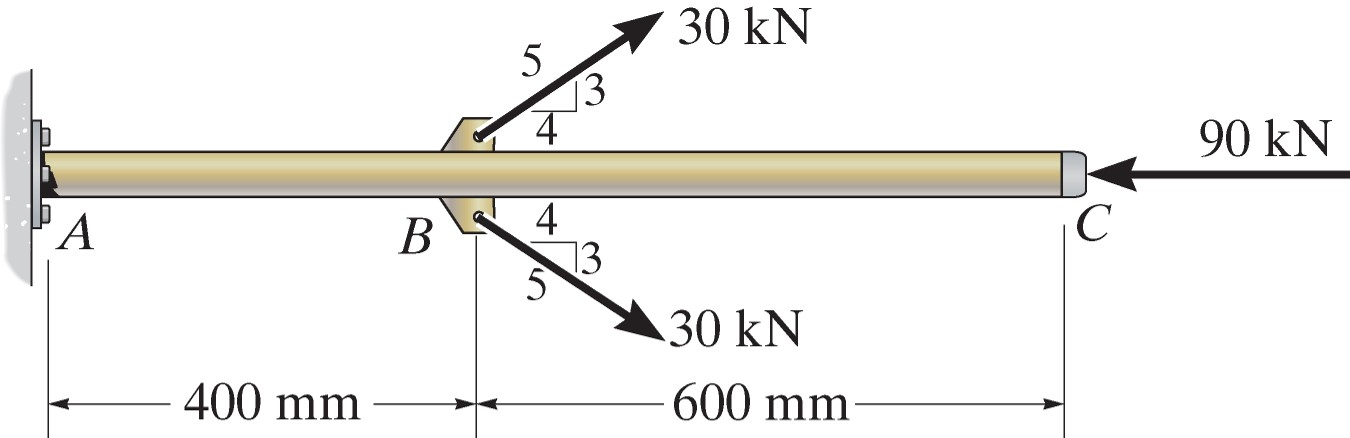
\includegraphics[width=0.8\linewidth]{f4-3}
		\end{figure}
		\textbf{Solution:} To find the displacement at $C$ we need to find the total displacement of the rod.
		To do that we will need to add the effects of the loading at $B$ with the loading at $C$.
		\begin{itemize}
			\item We can start by finding the displacement between $AB$, $\delta_{AB} = \frac{(2)(\SI{30}{kN})(4/5)(\SI{400}{mm})}{(\pi (\SI{15}{mm})^2)(\SI{200 }{GPa})} = \SI{0.136}{mm}$
			\item And we add to that the displacement from the compressive force at $C$, $\delta_{AC} = \frac{(\SI{-90}{kN})(\SI{1000}{mm})}{(\pi (\SI{15 }{mm})^2)(\SI{200}{GPa})} = \SI{-0.637}{mm}$
			\item And the total displacement at $C$ is $\delta_C = \delta_{AB} + \delta_{AC} = \SI{-0.501}{mm}$
		\end{itemize}

	\item %4-11
		The load is supported by four stainless steel wires that are connected to rigid members $AB$ and $DC$.
		Determine the vertical displacement of the $\US{500}{lb}$ load if each wire has a cross-sectional area of $\US{.035}{in^2}$.
		\begin{figure}[H]
			\centering
			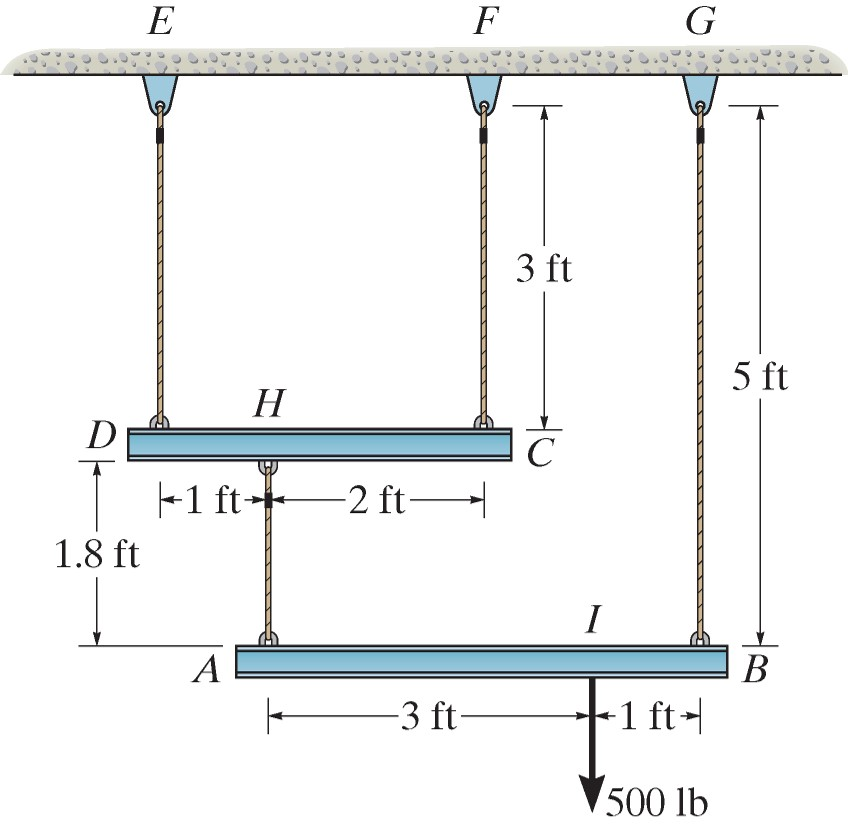
\includegraphics[width=0.5\linewidth]{4-11}
		\end{figure}
		\textbf{Solution:}
		\begin{itemize}
		\item First we need to do some statics to find the force in each wire.
			We find (see image for FBD) that $A=\US{125}{lb}$, $G=\US{375}{lb}$, $E=\US{83.3}{lb}$, and $F=\US{41.7}{lb}$
			\begin{figure}[H]
				\centering
				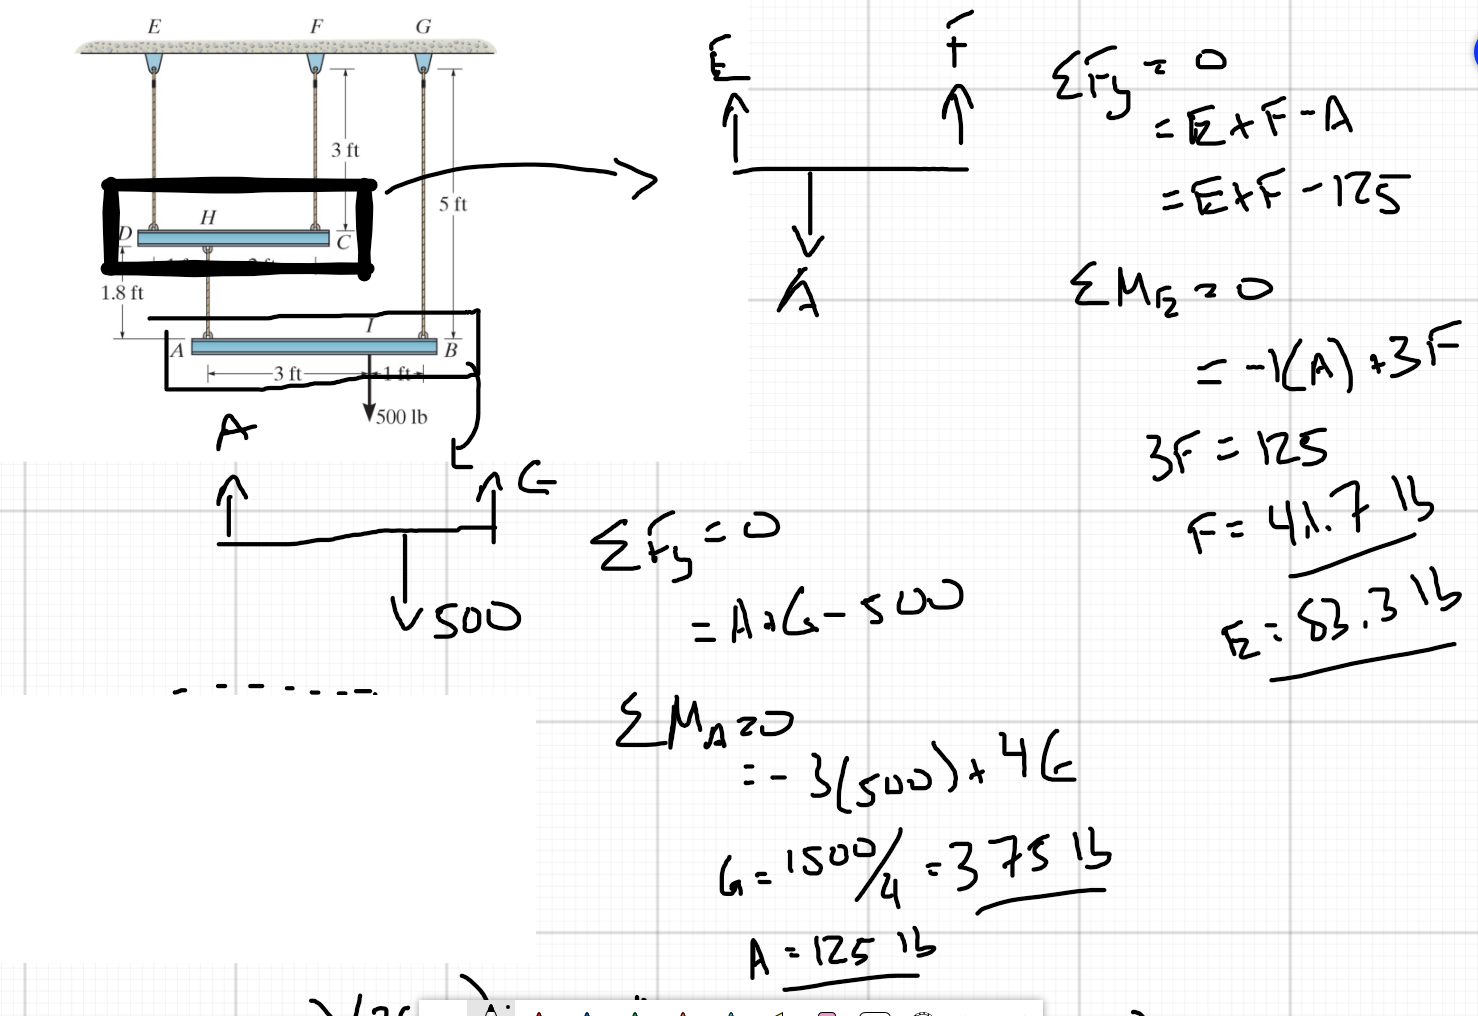
\includegraphics[width=0.7\linewidth]{2a}
			\end{figure}
		\item Next we need to find the amount each wire stretches using the deflection formula ($\delta = NL/AE$).
			We find $\delta_d = \US{0.00306}{in}$, $\delta_C = \US{0.00153}{in}$, $\delta_a = \US{0.00276}{in}$, and $\delta_b = \US{0.0230}{in}$
		\item We need to use similar triangles to find the displacement at $H$ and add that to the deflection at $A$, then use similar triangles again to find the displacement of the force at $I$ (see figure), note that I use $\delta$ to mean deflection due to wire stretch and a capital $\Delta$ to signify the actual displacement of a point (at $A$ we need both wire deflection and movement of the point $H$ to get the total displacement).
			\begin{figure}[H]
				\centering
        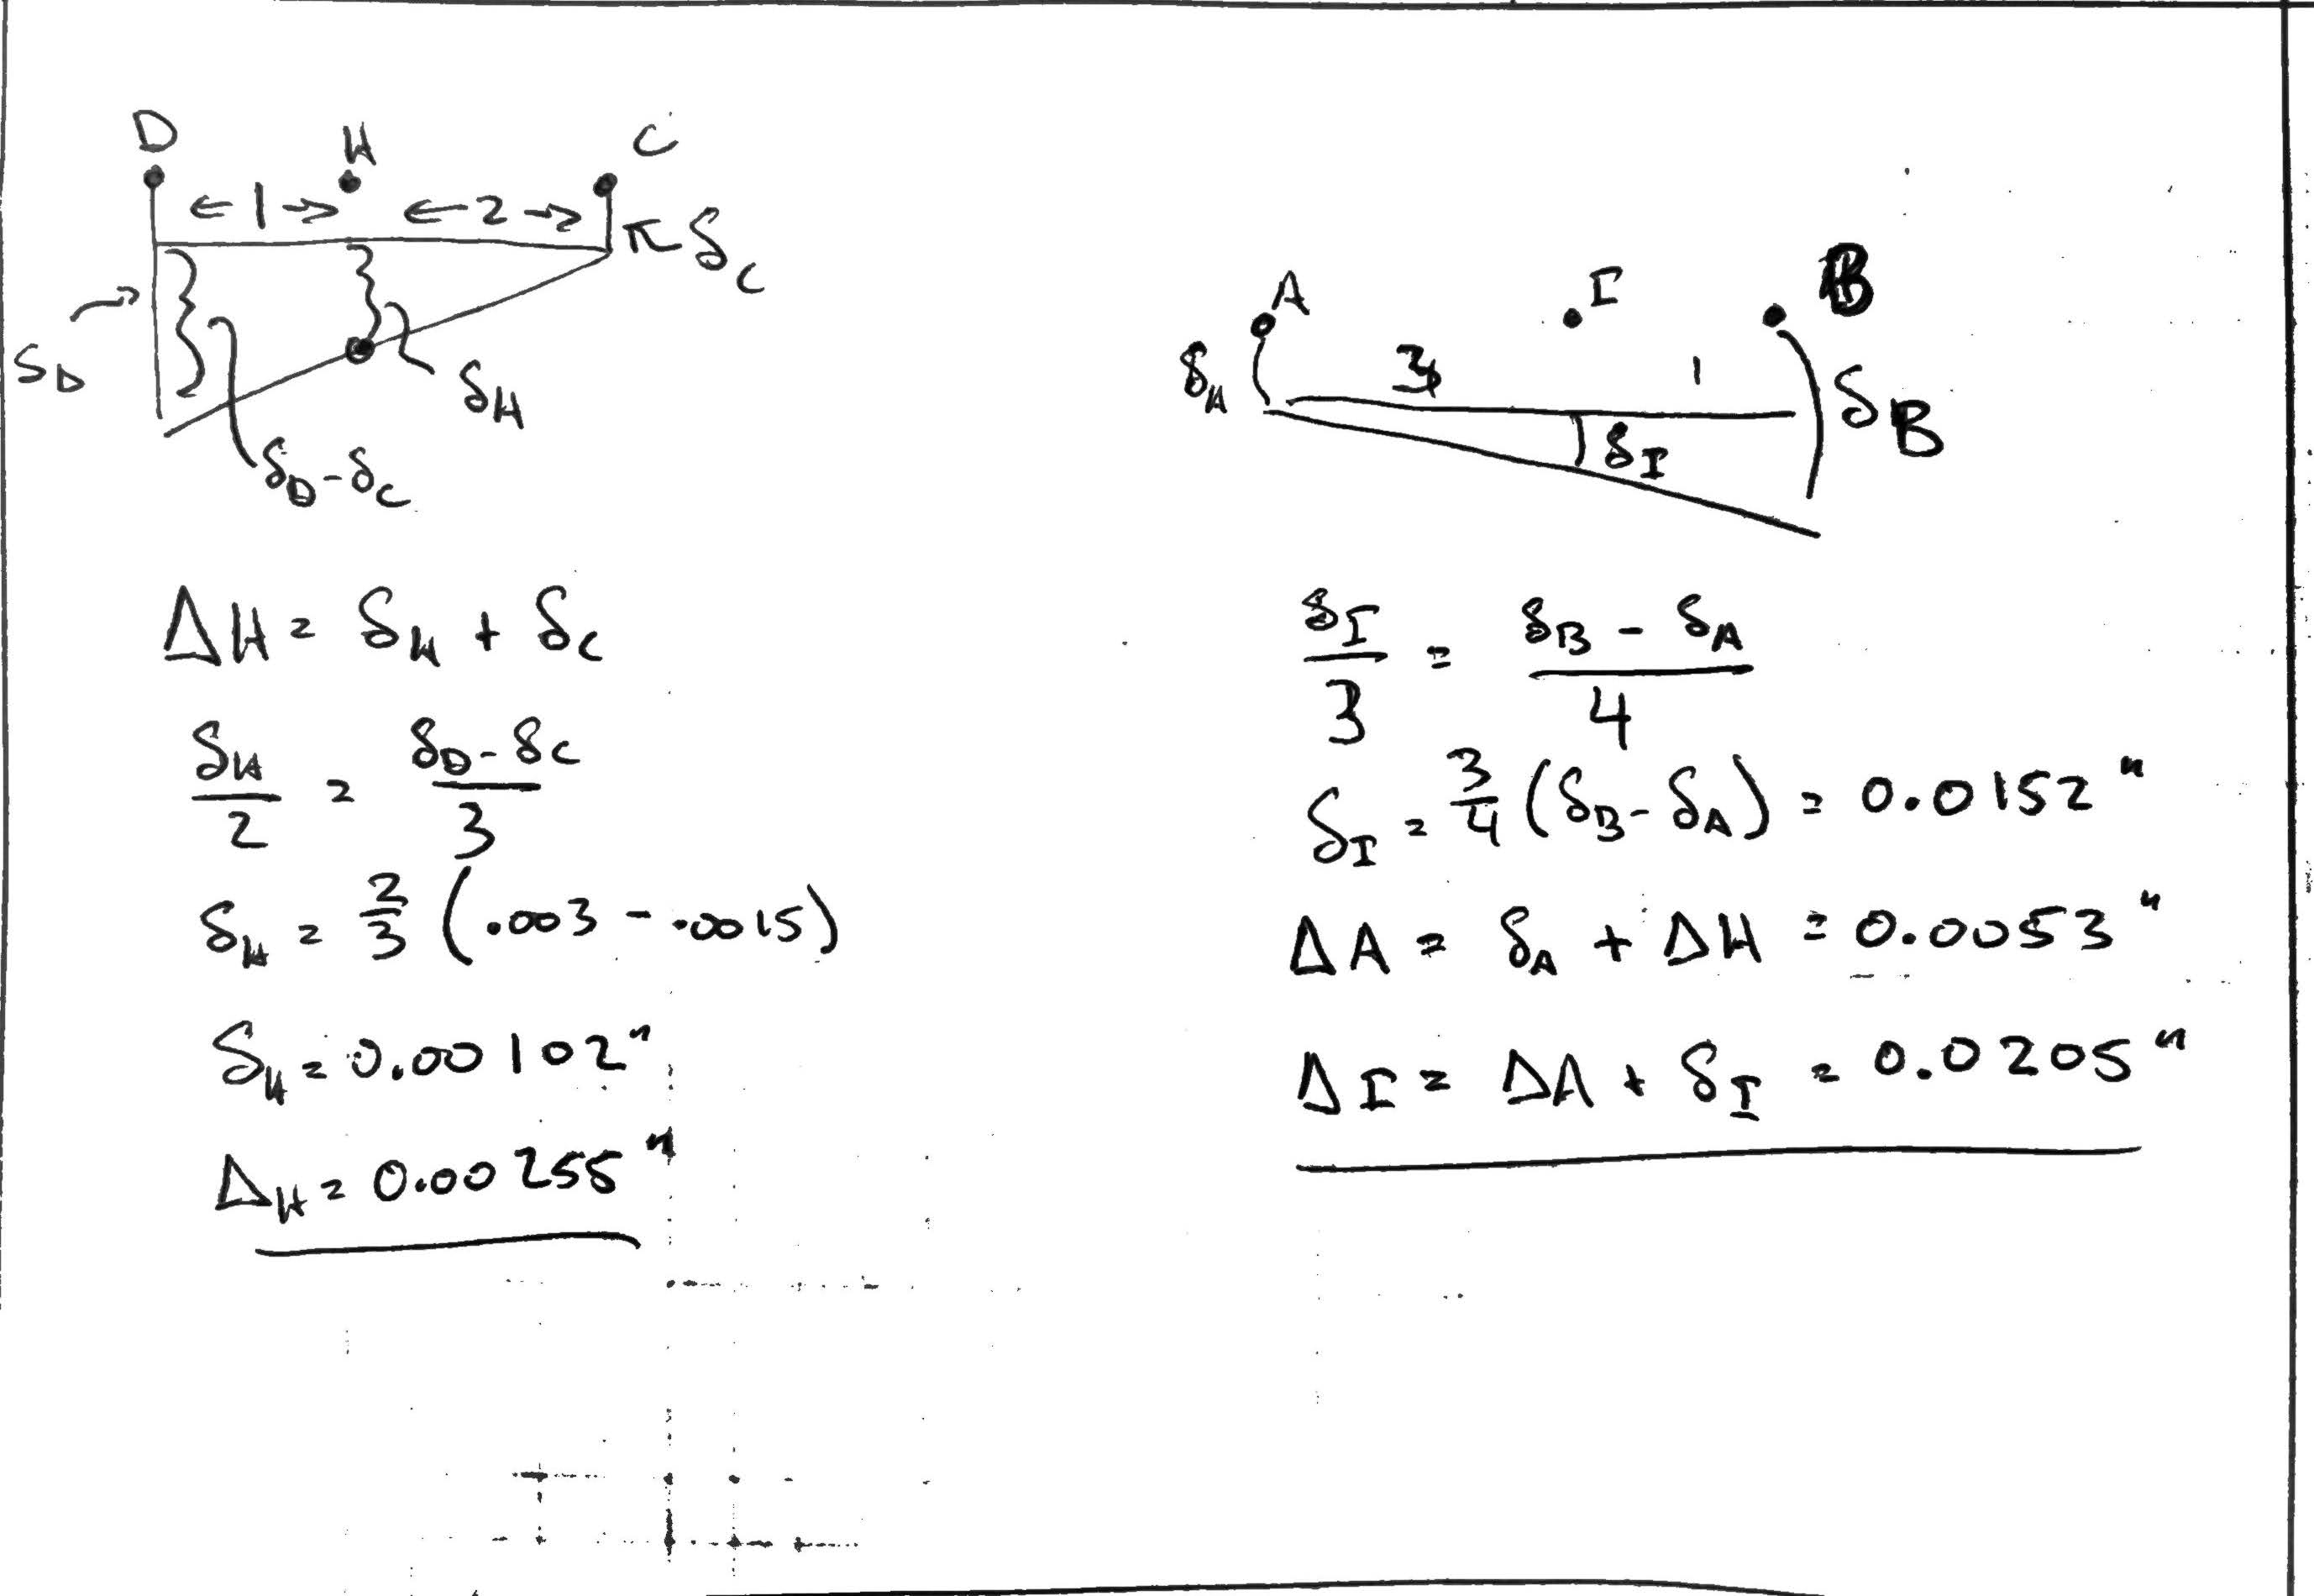
\includegraphics[width=0.8\linewidth]{2b-fixed}
			\end{figure}
	\end{itemize}

	\item %4-32
		The column shown is constructed from concrete with A992 steel rebar.
		If the column is subjected to an axial force of $\US{200}{kip}$, find the required rod diameter such that 60\% of the axial force is carried by the concrete.
		\begin{figure}[H]
			\centering
			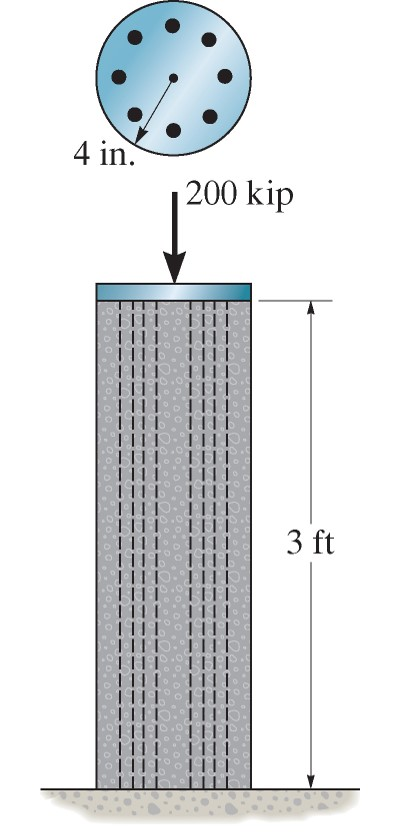
\includegraphics[width=0.25\linewidth]{4-32}
		\end{figure}
		\textbf{Solution:}
		\begin{itemize}
			\item We know that the concrete and the steel rebar need to displace by the same amount, but we don't know how much that is
			\item We do know, however, how much load should be carried by each member, this means that $\frac{N_{st}L}{A_{st}{E_{st}}} = \frac{N_{c}L}{A_{c}{E_{c}}} $
      \item The length is the same, so that can be canceled, we just need to solve for the area, note that $A_c = \pi 4^2 - A_{st}$, so this leaves us with $ \frac{N_{st}E_c}{N_c E_{st}} = \frac{A_{st}}{16 \pi - A_{st}} $
      \item Substituting $N_{st} = \US{80}{kip}$, $N_c = \US{120}{kip}$, $E_c = \US{3.2}{Msi}$ and $E_{st} = \US{29}{Msi}$ we find $A_{st} = \US{3.44}{in^2}$ which gives a steel rod diameter of $d = 2 \sqrt{\left( \frac{3.44}{8 \pi} \right)} = \US{0.740}{in}$.
		\end{itemize}
	
	\item %4-59
		The post is made from 2024 aluminum and has a diameter of $\SI{50}{mm}$.
		It is fixed at $A$ and $B$ and has a coiled spring attached to a rigid collar at $C$.
		If the spring is initially uncompressed, find the compression in the spring when a load of $P = \SI{75}{kN}$ is applied to the collar.
		\begin{figure}[H]
			\centering
			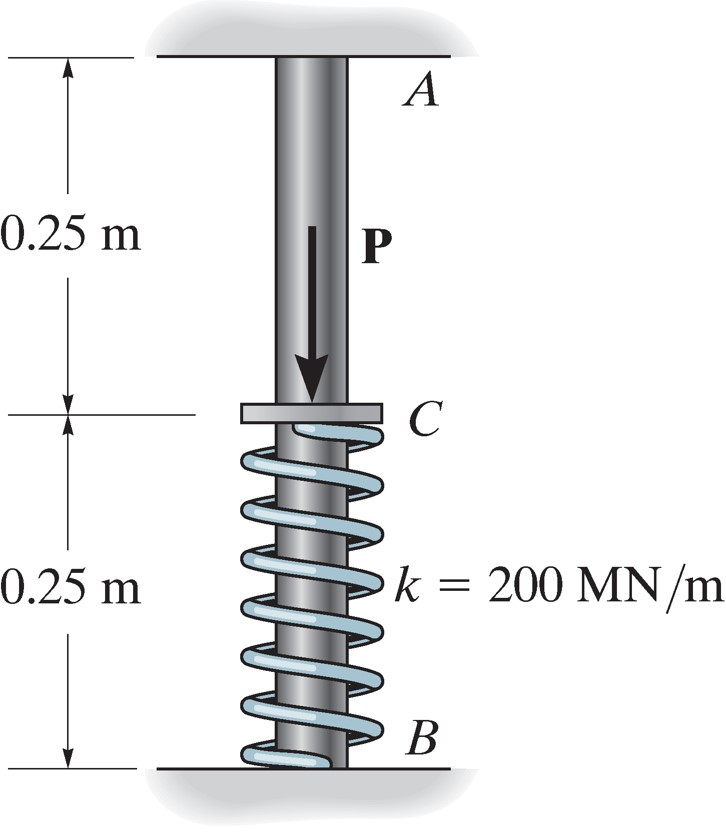
\includegraphics[width=0.45\linewidth]{4-59}
		\end{figure}
		\textbf{Solution:}
		\begin{itemize}
			\item In this solution we will use the method of sections, we will have three unknown internal forces in this problem, the internal force between $A$ and $C$ ($F_{AC}$), the internal force between $C$ and $B$ ($F_{BC}$) and the force in the spring, $F_s$.
			\item All of these forces need to add to the applied load $P$, and all will influence deflection at $C$, which needs to be equal, thus we have $\delta_c (F_{AC}) = \delta_c (F_{BC}) = \delta_c (F_s)$
			\item Substituting deflection relationships for axial loading and springs gives $ \frac{F_{AC} L_{AC}}{AE} = \frac{F_{BC}L_{BC}}{AE} = \frac{F_s}{k} $
      \item Since $L_{AC} = L_{BC}$ and $AE$ is constant, we can say that $F_A = F_C$, we can also relate $F_s$ to $F_A$ with $F_s = \frac{kF_{AC} L_{AC}}{AE}$ and finally we substitute into $F_{AC} + F_{BC} + F_s = P$ to find $ F_{AC}\left( \frac{k L_{AC}}{AE} \right) + F_{BC} + F_{AC} = P = F_{AC}\left(\frac{k L_{AC}}{AE} + 2 \right)$
			\item And we find that $F_{AC} = \SI{31.7}{kN}$ and $F_s = \SI{11.5}{kN}$ which gives a spring compression of $ \delta_c = F_s / k = \SI{0.058}{mm} $
			\item As a quick sanity check, we can compare the effective spring constant of the aluminum rod ($L/AE$) to the spring constant for the spring, we find that $k_{al} = \SI{550}{MN/m}$, and it makes sense then that the force in the aluminum is so much higher than the spring for the same deflection
		\end{itemize}

	\item %4-69
		The assembly has shown fits snugly with no internal force at $70 ^\circ F$.
		Find the average normal stress in each material when the temperature is raised to $200 ^\circ F$.
		\begin{figure}[H]
			\centering
			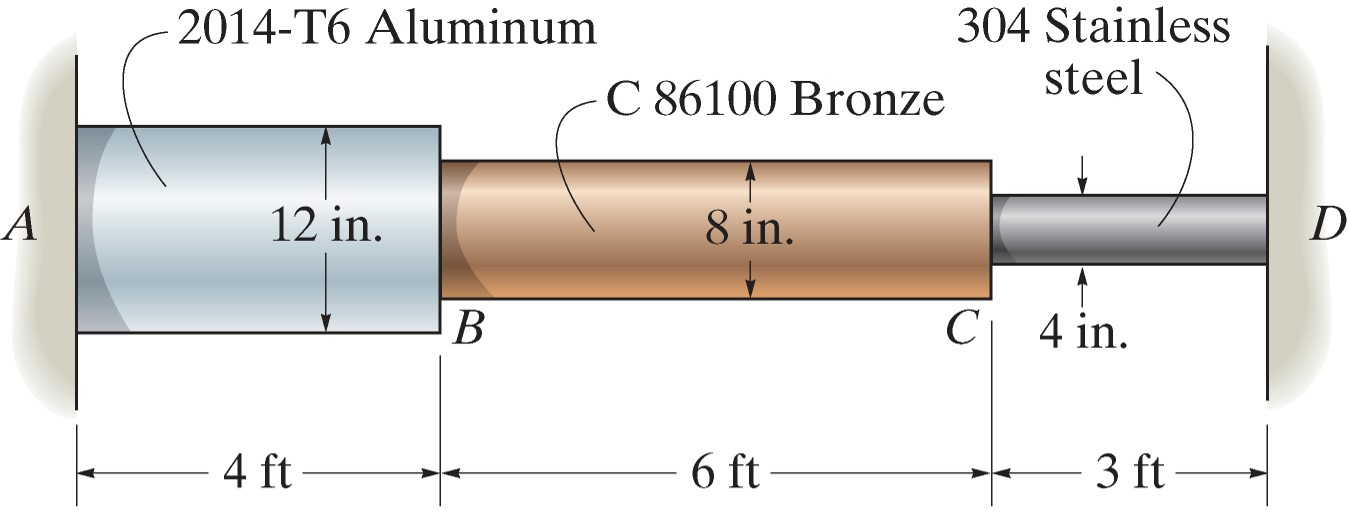
\includegraphics[width=0.8\linewidth]{4-69}
		\end{figure}
		\textbf{Solution:}
		\begin{itemize}
			\item For this problem we will use the force method and begin by neglecting the fixed support at $D$.
			\item With no support at $D$ each material can expand freely, with$\delta = \alpha \Delta T L$, we use $\alpha_{al} = 12.8\times 10^{-6}/^\circ F$, $\alpha_{br} = 12.2\times 10^{-6}/^\circ F$, and $\alpha_{st} = 9.6\times 10^{-6}/^\circ F$
			\item Substituting lengths (converted to inches), we find $\delta_{al} = \US{0.080}{in}$, $\delta_{br}=\US{0.114}{in}$, and $\delta_{st} = \US{0.045}{in}$ for a total thermal deflection of $\delta_T = \US{0.239}{in}$
			\item We need a reaction force to cancel this deflection exactly. From the method of sections, we can clearly see that the reaction force will also be exactly equal to the internal normal force in each material. Thus we need $\delta_M = \delta_T = \frac{N L_{al}}{E_{al}A_{al}} + \frac{N L_{br}}{E_{br}A_{br}} + \frac{N L_{st}}{E_{st}A_{st}}$
			\item Solving, we find $N = \US{1070}{kip}$ and this gives stresses of $\sigma_{al} = \US{9.46}{ksi}$, $\sigma_{br} = \US{21.3}{ksi}$ and $\sigma_{st} = \US{85.1}{ksi}$
		\end{itemize}

	\item %4-70
		The rod shown is made from aluminum and has a diameter of $\US{0.25}{in}$.
		If the rod is $\US{4}{ft}$ long when the springs are compressed $\US{0.5}{in}$ and the temperature of the rod is $40 ^\circ F$, find the force in the rod when the temperature is $150 ^\circ F$.
		\begin{figure}[H]
			\centering
			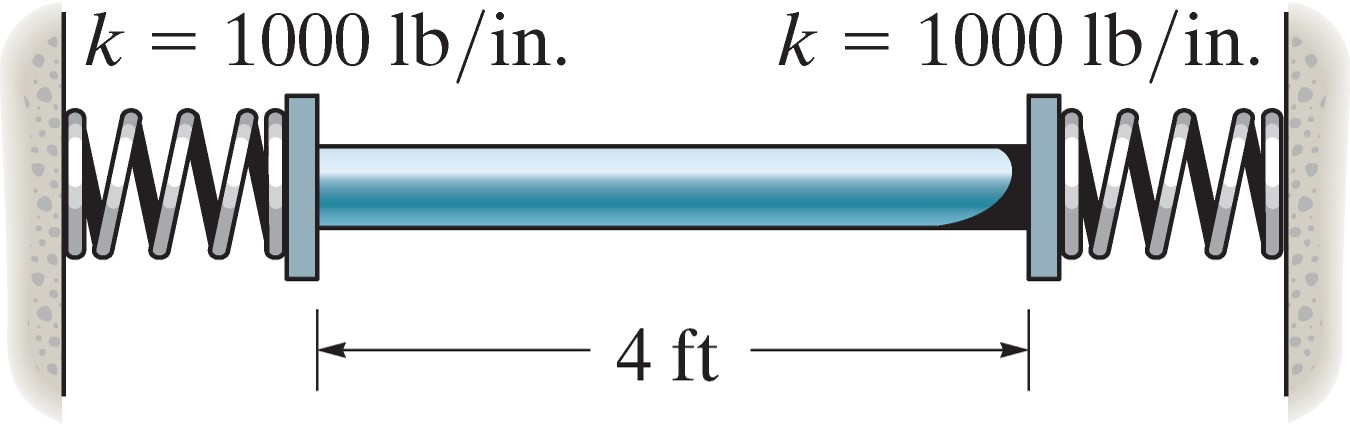
\includegraphics[width=0.8\linewidth]{4-70}
		\end{figure}
		\textbf{Solution:}
		\begin{itemize}
			\item We can simplify this problem slightly by considering the symmetry, we will consider the center to be the axis of symmetry, where there will be no displacement.
			\item For this problem, we will use the method of sections. We are given that before any thermal expansion, there is some compression in the springs, which will put some force into the aluminum, but since it is in equilibrium we can neglect it for now.
			\item Additional displacement will have a thermal and mechanical component for the aluminum, $\delta = \delta_T + \delta_M = x$ which will also equal the additional displacement $x$ in the spring, since $F=kx$ we can say that $\delta_T + \delta_M = F_s/k$
			\item The normal force in the aluminum must be equal and opposite to the force in the spring, so we can further say that $\delta_T - \frac{F_s L}{AE} = \frac{F_s}{k} $
			\item Substituting values we find that $F_s = \US{19.7}{lb}$, the total force in the rod however will also include $\US{500}{lb}$ from the initial spring compression, giving $F_s = N = \US{520}{lb}$
		\end{itemize}

	\item %4-76
		The device shown is used to measure temperature.
		Bars $AB$ and $CD$ are made of tungsten ($\alpha = 4.5 \times 10^{-6} \text{ } ^\circ C^{-1}$) and aluminum ($\alpha = 23 \times 10^{-6} \text{ } ^\circ C^{-1}$), respectively.
		At room temperature ($20^\circ C$) the rigid bar $AE$ is horizontal.
		Find the vertical displacement of the pointer when the temperature is $200 ^\circ C$.
		\begin{figure}[H]
			\centering
			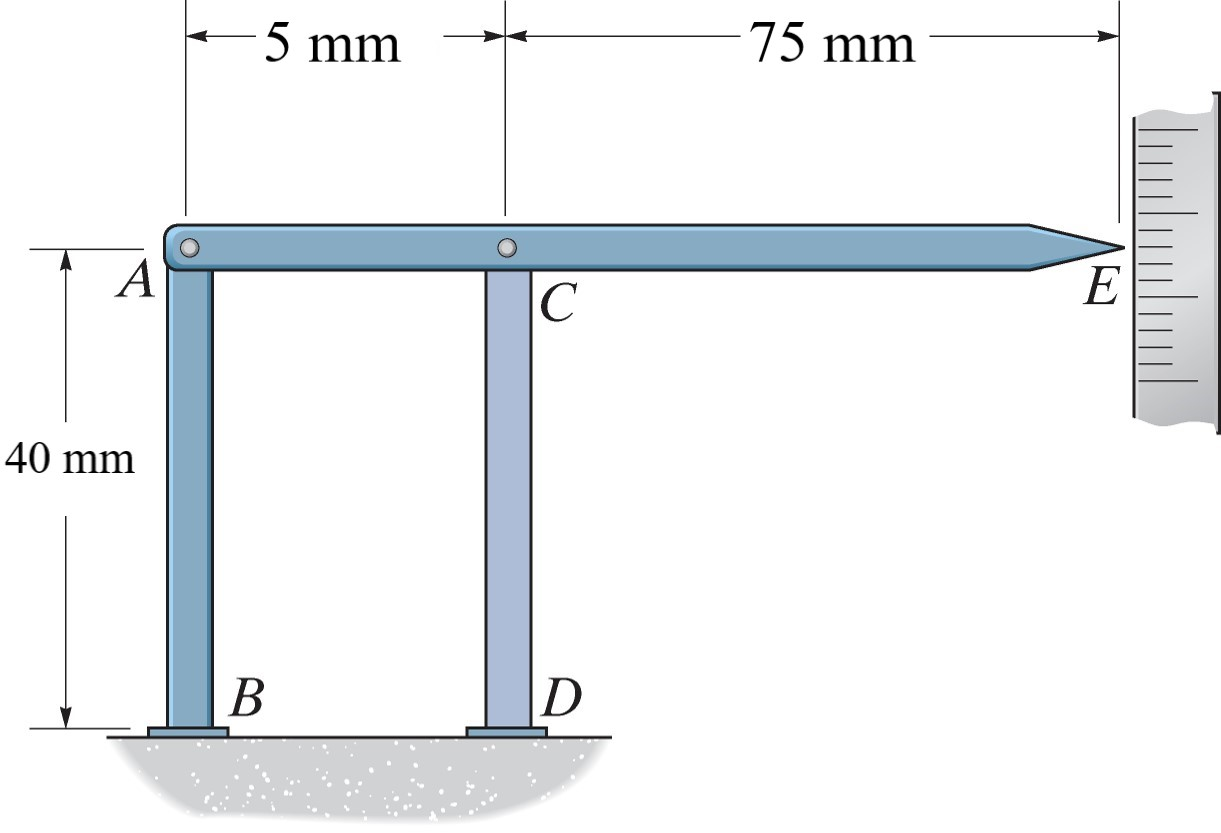
\includegraphics[width=0.8\linewidth]{4-76}
		\end{figure}
		\textbf{Solution:}
		\begin{itemize}
			\item We can use similar triangles to relate the displacement at the scale to the thermal displacement in each of the legs, see figure
				\begin{figure}[H]
					\centering
					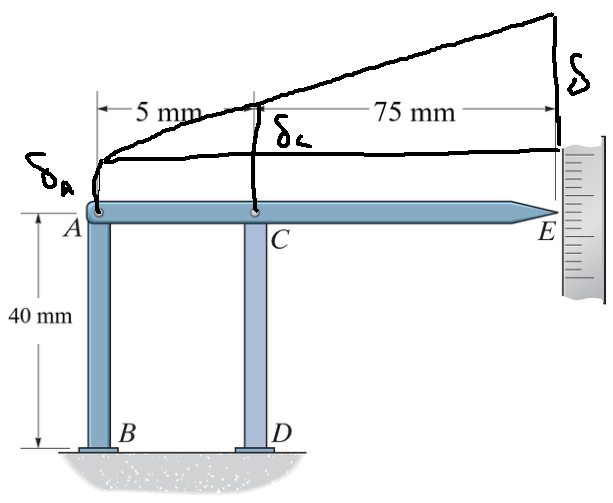
\includegraphics[width=0.6\linewidth]{7}
				\end{figure}
			\item We also need to add the total shift (below the triangle), so our final expression is $\delta = \delta_a + \frac{80(\delta_c-\delta_a)}{5}$
			\item Substituting known values we find $\delta = \SI{2.16}{mm}$
		\end{itemize}

\end{enumerate}
\end{document}
